\documentclass[a4paper,11pt]{article}
\usepackage[utf8]{inputenc}
\usepackage[draft]{graphicx}  % disables actual image inclusion

%\usepackage{graphicx}
\usepackage{listings}
\usepackage{color}
\usepackage{geometry}
\usepackage{titlesec}
\usepackage{fancyhdr}
\usepackage{hyperref}

\geometry{margin=1in}
\pagestyle{fancy}
\fancyhf{}
\rhead{IAM Automation Lab}
\lhead{GT Programming Ops}
\cfoot{\thepage}

\titleformat{\section}{\Large\bfseries}{\thesection}{1em}{}
\titleformat{\subsection}{\normalsize\bfseries}{\thesubsection}{1em}{}

\definecolor{lightgray}{gray}{0.95}

\lstset{
  backgroundcolor=\color{lightgray},
  basicstyle=\ttfamily\small,
  frame=single,
  breaklines=true,
  postbreak=\mbox{\textcolor{red}{$\hookrightarrow$}\space}
}

\title{\textbf{IAM Automation Lab Documentation}}
\author{Your Name \\ \texttt{your.email@example.com} \\ GT Programming Ops Challenge}
\date{\today}

\begin{document}

\maketitle

\section*{Lab Overview}
This lab aims to automate Identity and Access Management (IAM) tasks on a Linux machine using a Bash script. The script handles user and group provisioning, home directory configuration, password policies, and optional email notifications. All activities are logged for auditability.

\section*{Objectives}
\begin{itemize}
  \item Automate user and group creation from a CSV file.
  \item Assign full names and group memberships.
  \item Apply password complexity and enforce password resets.
  \item Secure each user's home directory.
  \item Log all actions to a file.
  \item Optionally send notification emails and validate password complexity.
\end{itemize}

\section*{Environment}
\begin{itemize}
  \item \textbf{OS}: Ubuntu 22.04 LTS
  \item \textbf{Tools}: \texttt{bash}, \texttt{useradd}, \texttt{groupadd}, \texttt{chage}, \texttt{passwd}, \texttt{mailutils}
  \item \textbf{Privileges}: Root or sudo required
\end{itemize}

\section*{Input File Format}
The script accepts a CSV file named \texttt{users.txt} in the following format:
\begin{lstlisting}
username,fullname,group
jdoe,John Doe,engineering
asmith,Alice Smith,engineering
mjones,Mike Jones,design
\end{lstlisting}

\begin{figure}[h!]
  \centering
  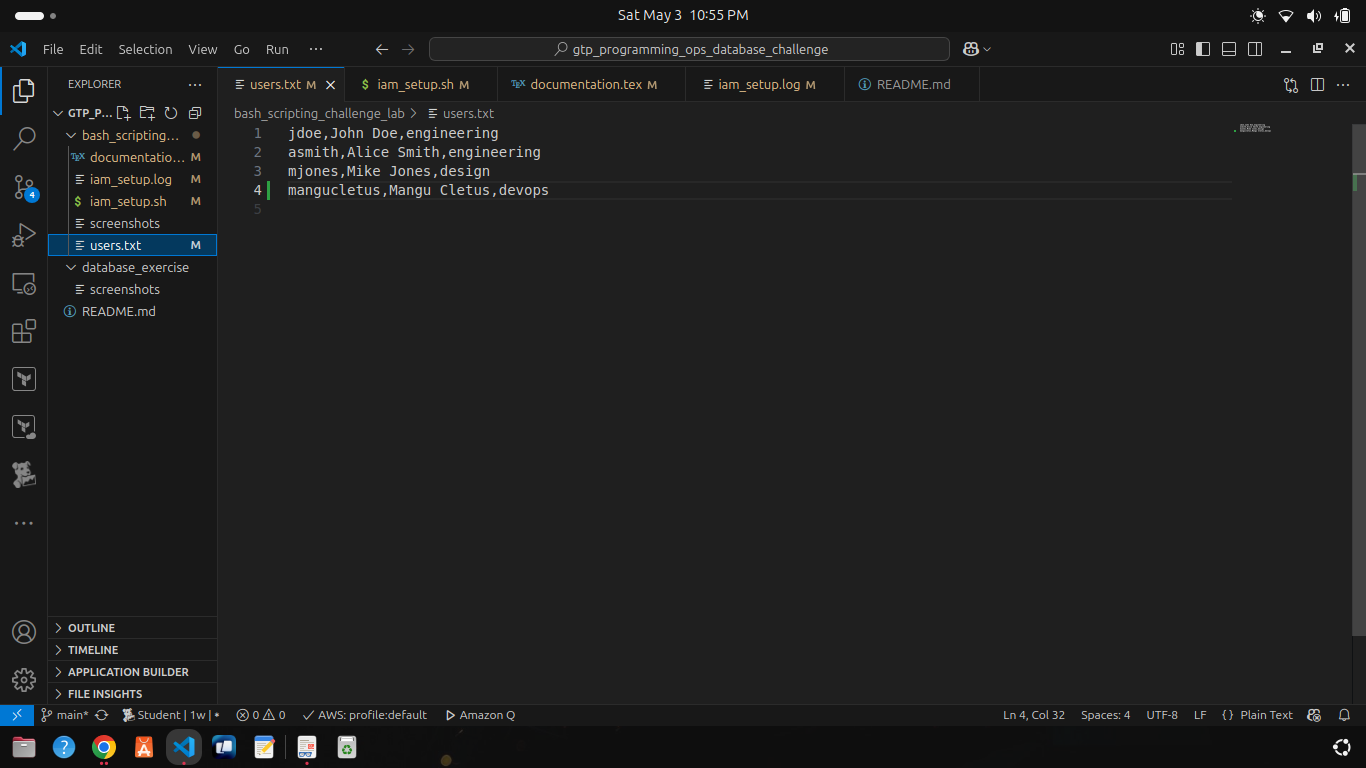
\includegraphics[width=0.6\textwidth]{screenshots/users_txt_content.png}
  \caption{Sample users.txt format}
\end{figure}

\section*{Script Overview: \texttt{iam_setup.sh}}

\subsection*{Main Features}
\begin{itemize}
  \item Checks and creates groups if they do not exist.
  \item Adds users with full name, group, home directory.
  \item Assigns temporary password and enforces reset.
  \item Validates password complexity.
  \item Locks down home directory permissions using \texttt{chmod 700}.
  \item Sends optional email notifications to users.
  \item Logs all actions to \texttt{iam_setup.log}.
\end{itemize}

\begin{figure}[h!]
  \centering
  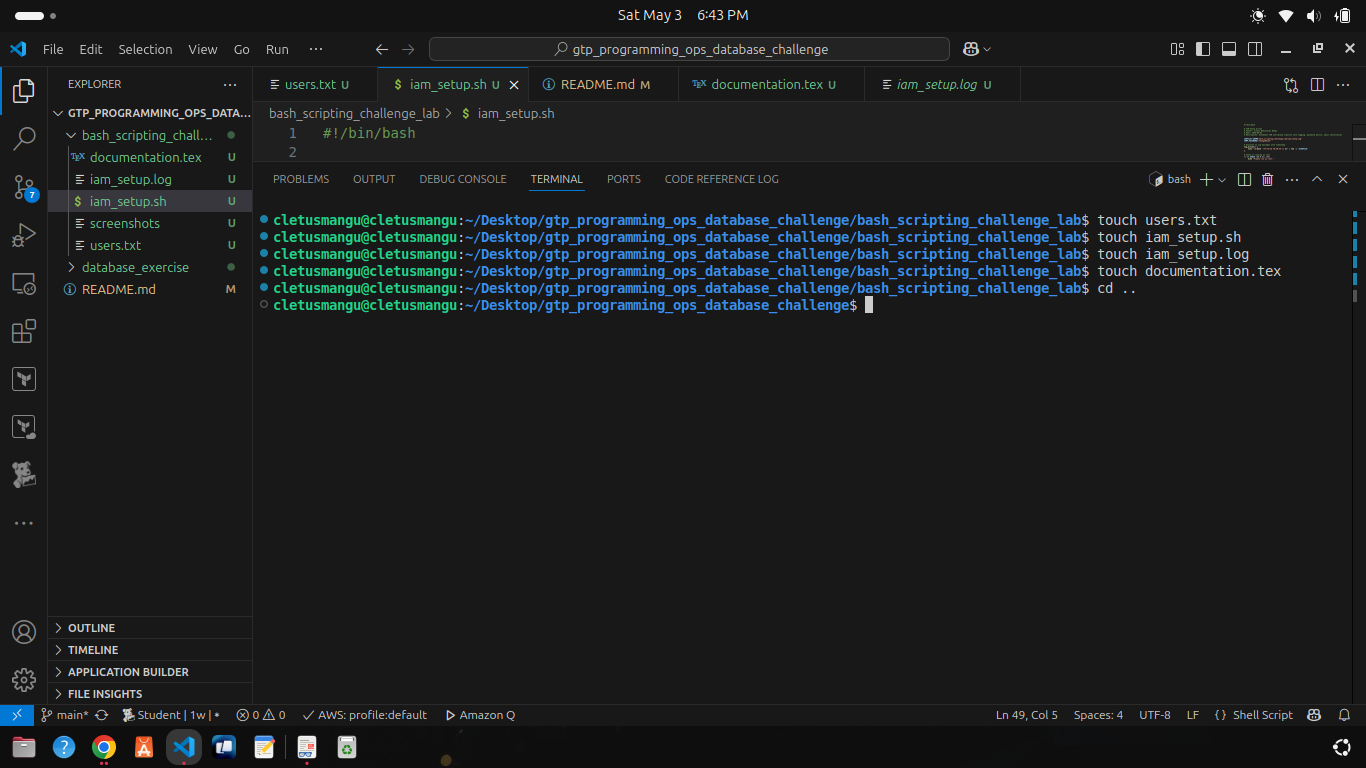
\includegraphics[width=0.7\textwidth]{screenshots/script_in_terminal.png}
  \caption{Script displayed in terminal}
\end{figure}

\section*{Running the Script}

\subsection*{1. Make Script Executable}
\begin{lstlisting}
chmod +x iam_setup.sh
\end{lstlisting}

\subsection*{2. Install Dependencies (Optional)}
\begin{lstlisting}
sudo apt update
sudo apt install mailutils -y
\end{lstlisting}

\subsection*{3. Execute the Script}
\begin{lstlisting}
sudo ./iam_setup.sh users.txt
\end{lstlisting}

\begin{figure}[h!]
  \centering
  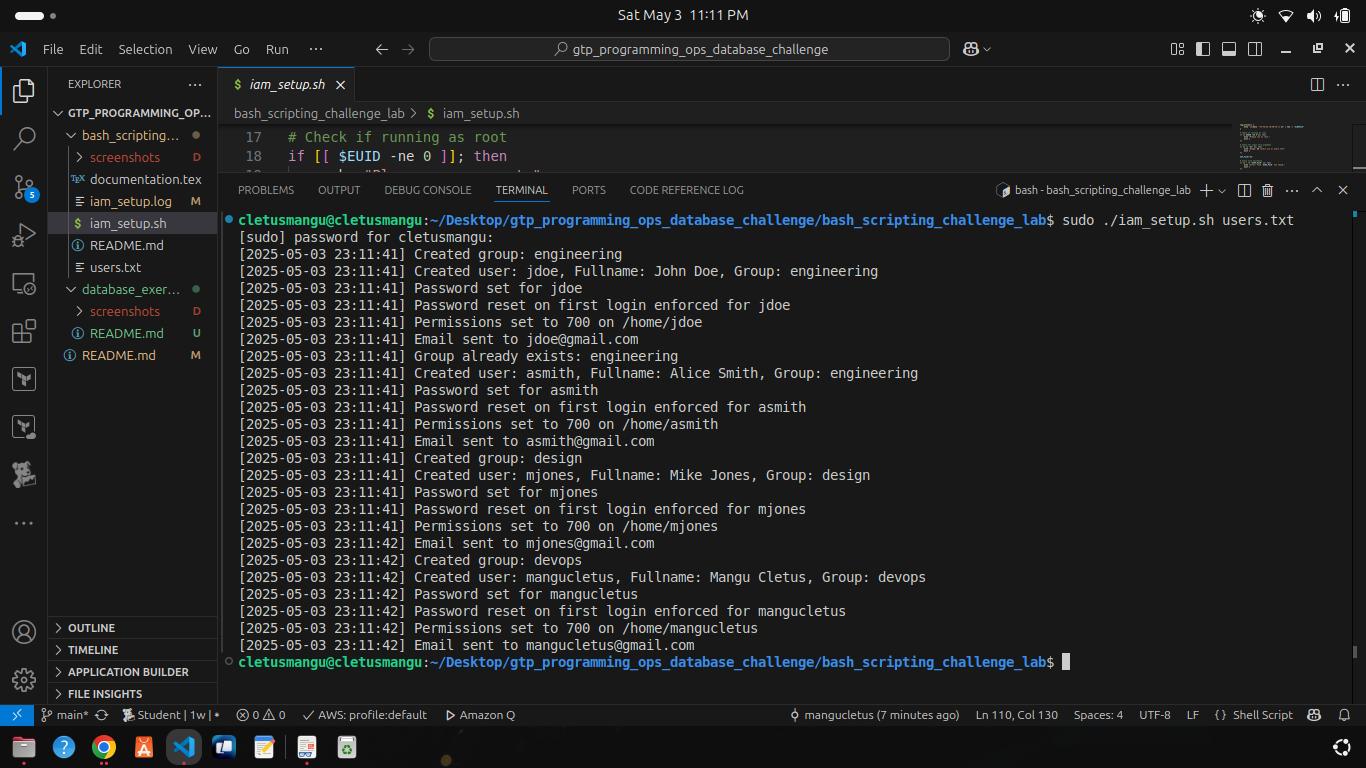
\includegraphics[width=0.7\textwidth]{screenshots/run_script.png}
  \caption{Executing the IAM script}
\end{figure}

\section*{Logging and Password Enforcement}

\subsection*{Logging}
All actions are recorded in \texttt{iam_setup.log}:
\begin{lstlisting}
[2025-05-03 14:20:12] Created group: engineering
[2025-05-03 14:20:14] Created user: jdoe
[2025-05-03 14:20:15] Set password for jdoe
\end{lstlisting}

\begin{figure}[h!]
  \centering
  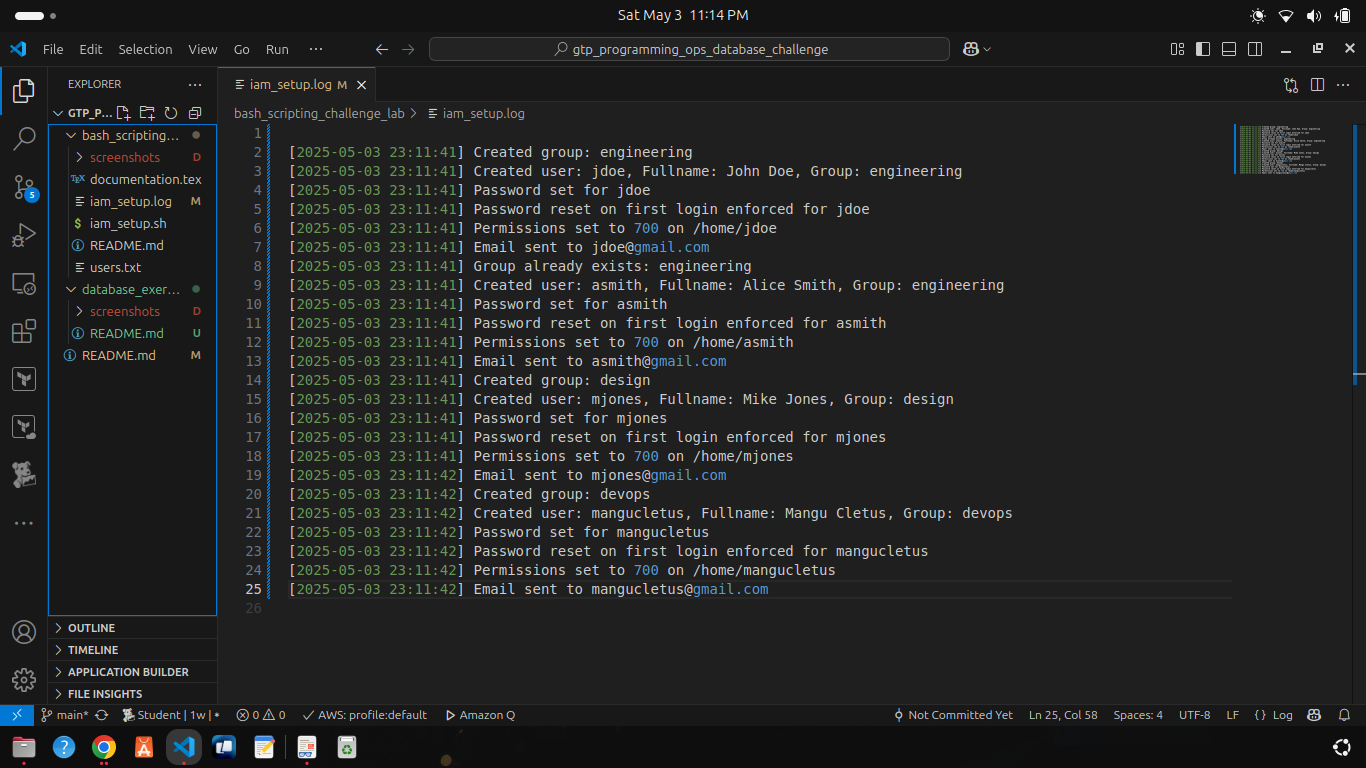
\includegraphics[width=0.65\textwidth]{screenshots/log_output.png}
  \caption{View of log file output}
\end{figure}

\subsection*{Password Policy}
The temporary password must meet:
\begin{itemize}
  \item Minimum 8 characters
  \item At least 1 uppercase, 1 lowercase, and 1 digit
\end{itemize}

\begin{lstlisting}
chage -d 0 username
\end{lstlisting}

\begin{figure}[h!]
  \centering
  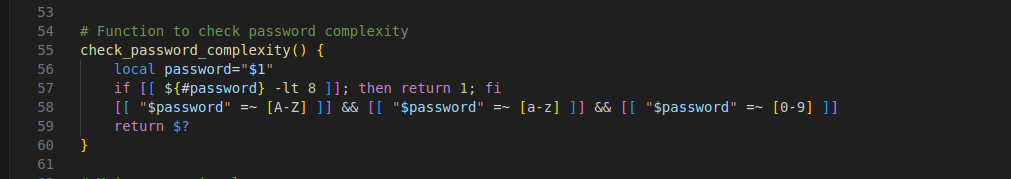
\includegraphics[width=0.65\textwidth]{screenshots/password_policy.png}
  \caption{Password policy applied and enforced}
\end{figure}

\section*{Permissions}
Each user's home directory is restricted:

\begin{lstlisting}
chmod 700 /home/username
\end{lstlisting}

\begin{figure}[h!]
  \centering
  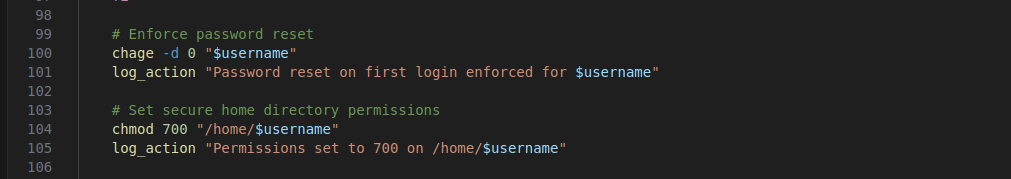
\includegraphics[width=0.6\textwidth]{screenshots/home_dir_permissions.png}
  \caption{Verifying permissions for home directory}
\end{figure}

\section*{Optional: Email Notification}

\begin{lstlisting}
echo "Welcome to the system, $FULLNAME." | mail -s "Account Created" $USERNAME@example.com
\end{lstlisting}

\begin{figure}[h!]
  \centering
  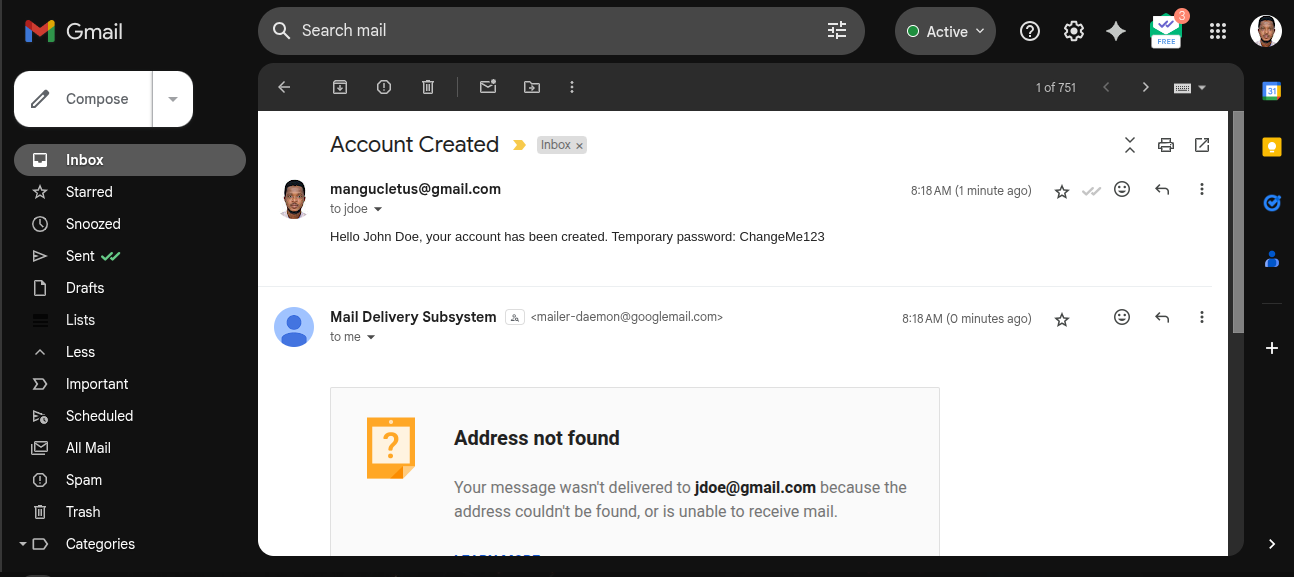
\includegraphics[width=0.65\textwidth]{screenshots/email_notification.png}
  \caption{Email notification sent from script}
\end{figure}

\section*{Project Directory Structure}
\begin{lstlisting}
iam_project/
├── iam_setup.sh
├── users.txt
├── iam_setup.log
├── README.md
└── screenshots/
    ├── users_txt_content.png
    ├── script_in_terminal.png
    ├── run_script.png
    ├── password_policy.png
    ├── log_output.png
    ├── home_dir_permissions.png
    └── email_notification.png
\end{lstlisting}

\section*{Submission}
\begin{itemize}
  \item Push your project to GitHub with:
    \begin{itemize}
      \item Script file
      \item users.txt
      \item log file
      \item screenshots
      \item README.md and this LaTeX file
    \end{itemize}
  \item Submit the GitHub repository link via the official form.
\end{itemize}

\section*{Author}
\textbf{Your Name} \\
Email: \texttt{your.email@example.com} \\
GitHub: \url{https://github.com/mangucletus}

\end{document}
